\chapter{相关理论与技术}\label{chap:theories_tech}

\section{Linux调度子系统}

% 内核Core调度流程
% 影响内核调度的关键因素
% - HZ
% - 调度类/机制
% - 调度策略/算法
% - 高质量的操作系统组件,如调度器,则可能需要数十年的时间来完善\citep{agache2020firecracker}

调度子系统是Linux内核的一个重要组成部分,负责在多任务场景中为每个任务分配CPU资源。Linux调度子系统在架构上可分为如图~\ref{fig:sched_arch}所示三层,每层为上层提供了基本机制,各层协作为复杂调度机制的实现提供了可能。最底层的Sched Core层提供了基本的调度框架,包括抢占调度与非抢占调度。Sched Class层提供了不同的调度机制,如实时调度、公平调度等。最高层的Sched Policy层提供了不同的任务调度逻辑,如FIFO(First In, First Out)、RR(Round Robin)。例如,Fair调度类在Core调度框架中的抢占式调度上实现了基于vruntime的调度机制,并提供NORMAL与BATCH两种调度策略,来控制不同优先级任务的vruntime积累速度。

\begin{figure}[!htbp]
    \centering
    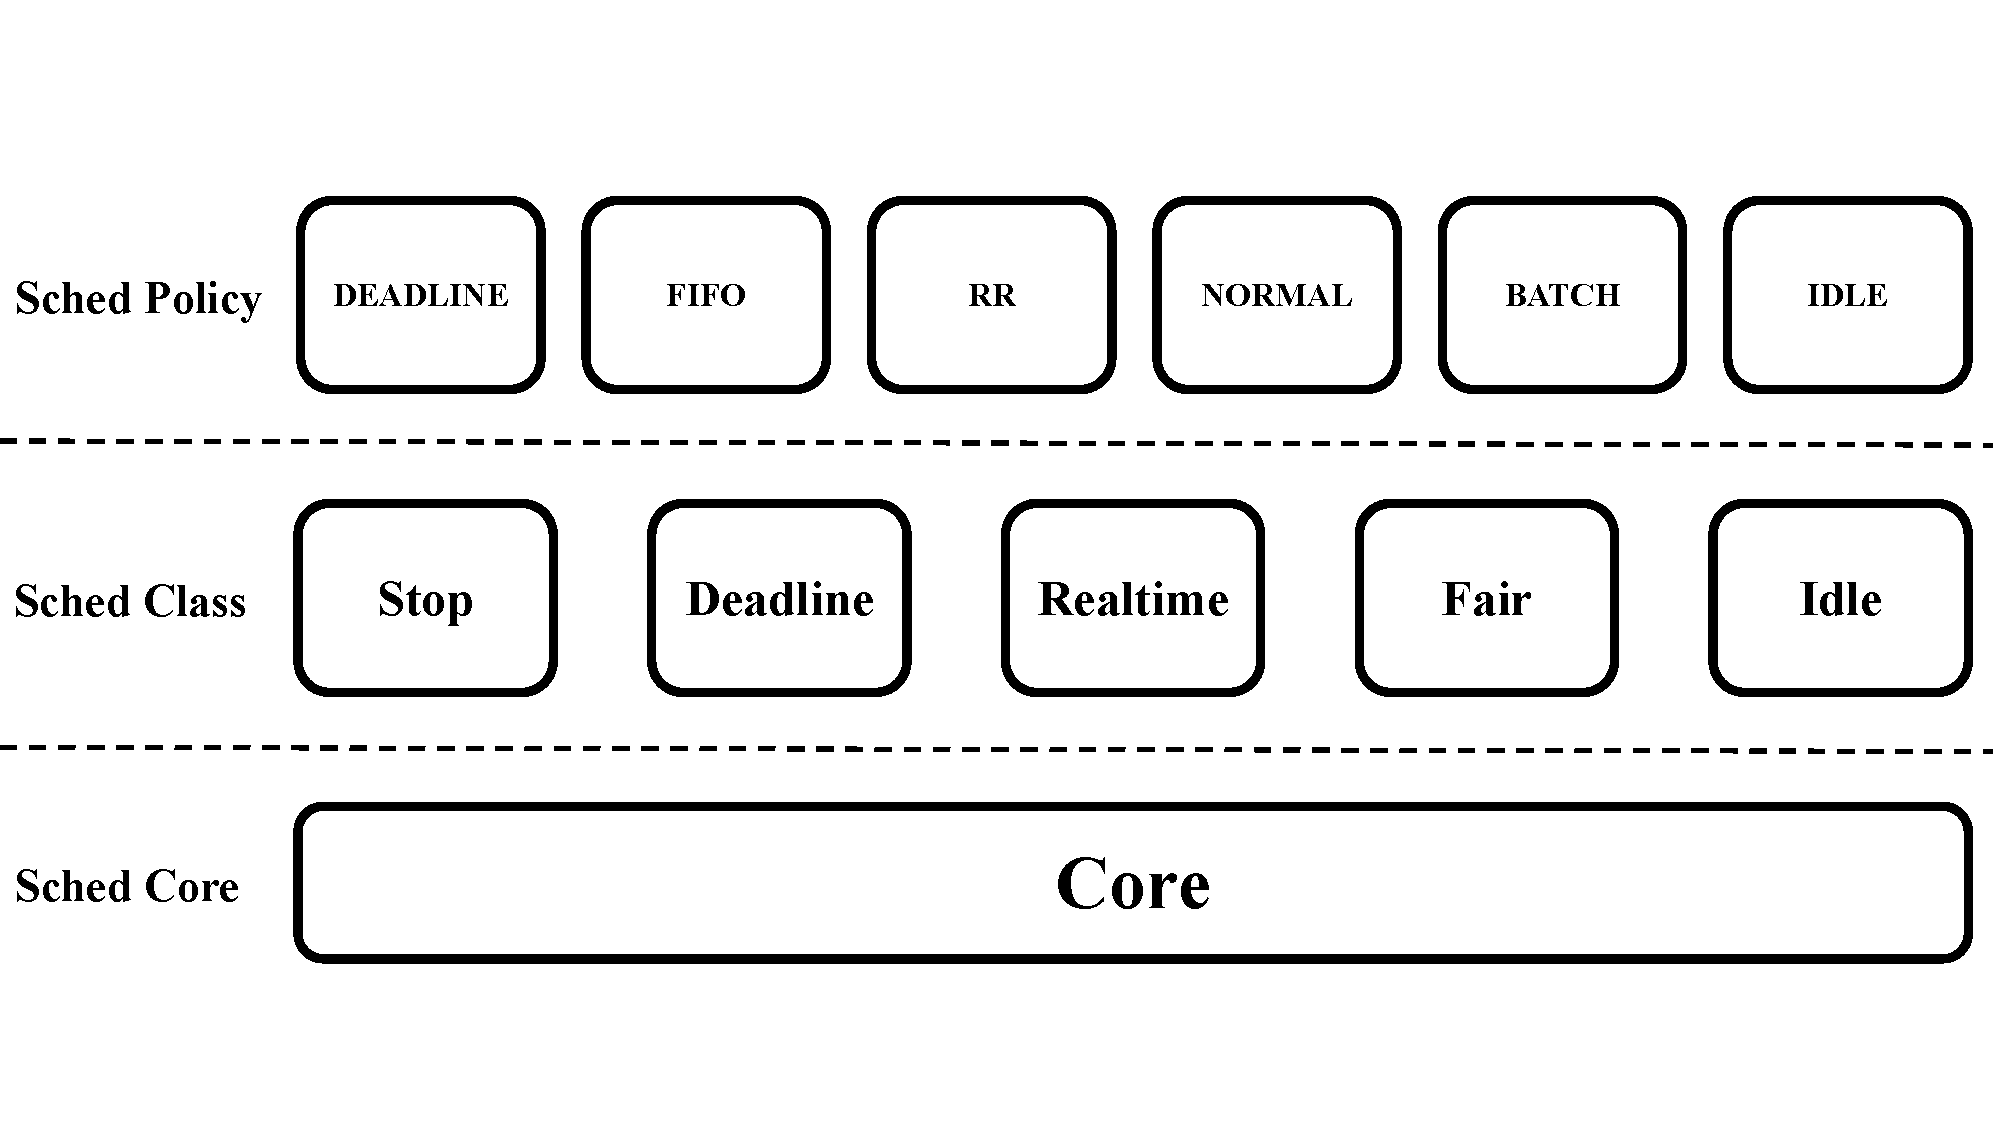
\includegraphics[width=0.7\textwidth]{sched_arch}
    \bicaption{\quad Linux调度子系统架构}{\quad Architecture of the Linux scheduling subsystem}
    \label{fig:sched_arch}
\end{figure}

\begin{itemize}

    \item Sched Core层作为最基本的调度框架,是所有调度类的入口。其中非抢占式调度源于批处理调度,该场景下任务依次执行直到退出。如图~\ref{fig:schedule_core}所示,非抢占式调度需要为新fork出来的任务选择合适的CPU,当任务主动出让CPU或退出时,再选择下一个任务并执行任务切换。任务切换的完整过程就是调度循环。如图~\ref{fig:shcedule_loop}所示,调度循环由中断和系统调用驱动,通常在返回用户态之前判断标志位来决定是否进入调度循环。抢占式调度基于CPU的分时复用,并由时钟中断驱动。如图~\ref{fig:schedule_tick}所示,在时钟中断处理中会进行task\_tick,包含处理当前任务所属调度类的相关回调函数,如更新记账信息、抢占决策等。抢占决策通过内核函数resched\_curr实现,通常仅设置抢占标志位并等待调度循环来完成抢占。

\begin{figure}[!htbp]
    \centering
    \begin{subfigure}[b]{0.42\textwidth}
        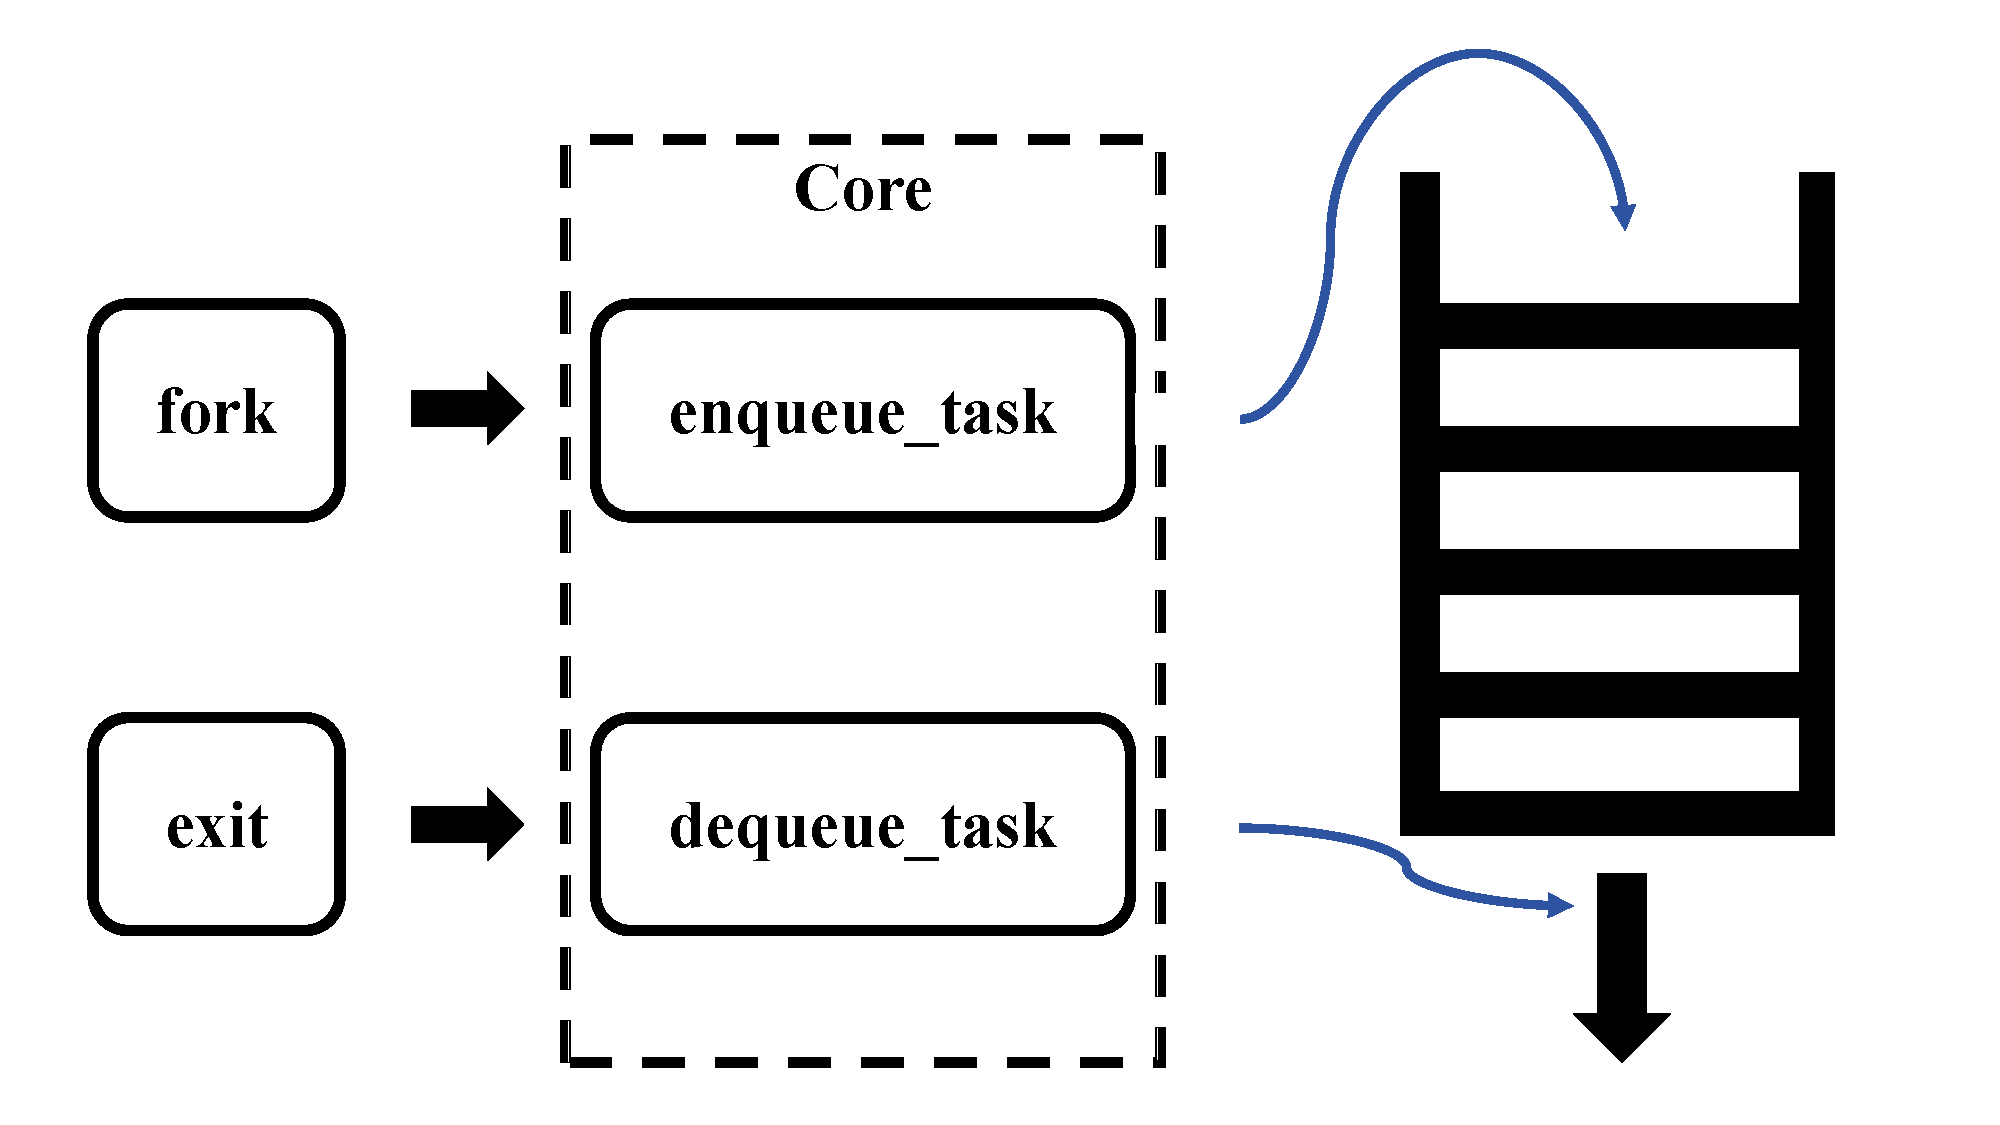
\includegraphics[width=\textwidth]{schedule_core}
        \caption{\quad 非抢占式调度}
        \label{fig:schedule_core}
    \end{subfigure}
    \hspace{0.5cm}
    \begin{subfigure}[b]{0.42\textwidth}
        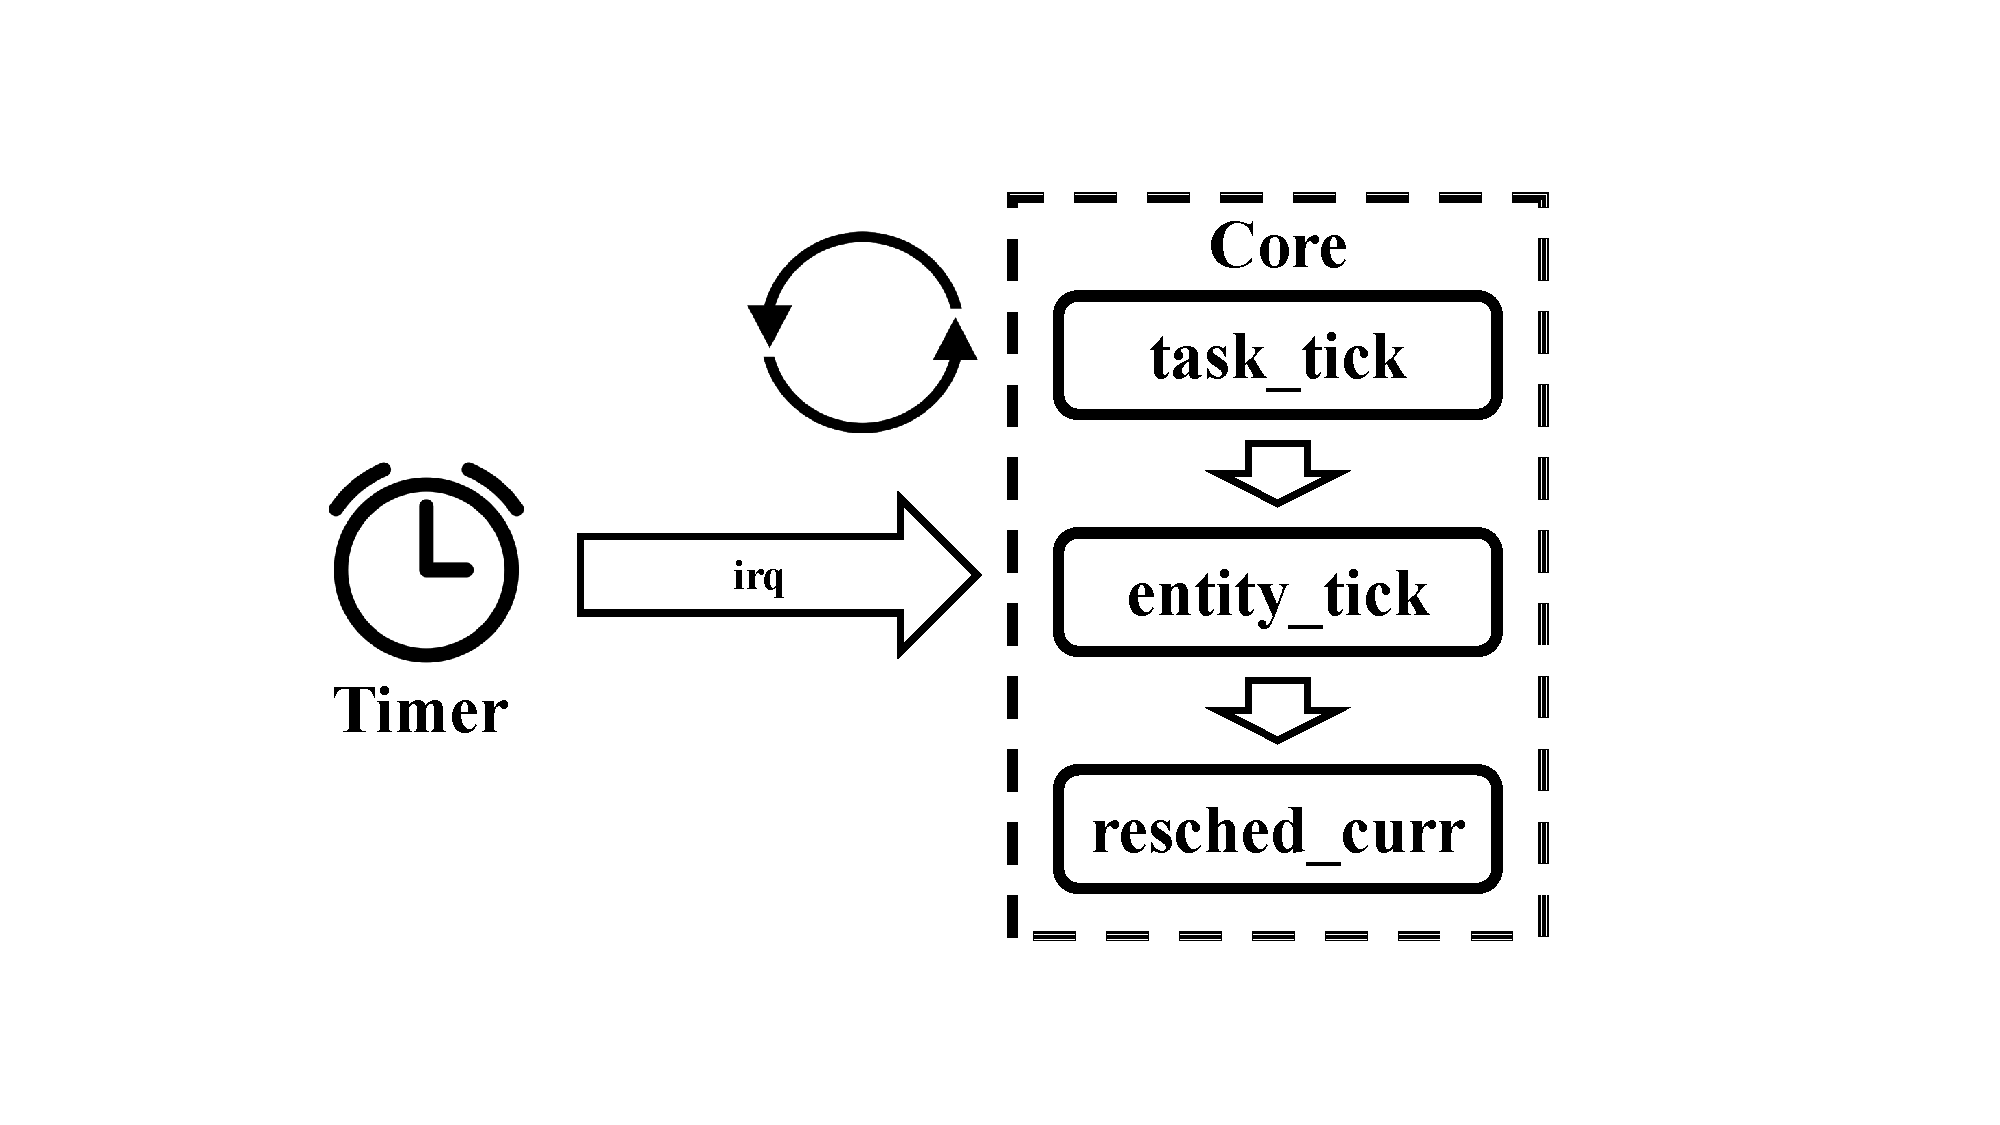
\includegraphics[width=\textwidth]{schedule_tick}
        \caption{\quad 抢占调度时钟滴答}
        \label{fig:schedule_tick}
    \end{subfigure}
    \bicaption{\quad 非抢占式调度与抢占式调度}{\quad Non-preemptive scheduling and preemptive scheduling}
    \label{fig:cpu_series_memcached}
\end{figure}

    \item Sched Class调度类层基于Core调度框架实现。当前Linux中主要包含Stop、Deadline、Realtime、Fair、Idle五种调度类\citep{scheduler}。其中,Stop调度类的实现最简单,其本质上是从批处理调度中提取出简单逻辑。Fair调度类最复杂,使用到如红黑树等高级数据结构,并采用了较复杂的启发式算法与记账逻辑。Fair调度类以公平作为调度的目标,由于在多数场景下的稳定性能,因此长久以来都是Linux中任务的默认调度类。其余调度类也有各自的设计目标,如Deadline调度类保证任务按固定的周期执行固定的时间,从而提供良好的实时性保证。调度子系统允许相同逻辑核上的任务属于不同的调度类,各调度类优先级如图~\ref{fig:sched_arch}所示从左向右逐渐降低。每个调度循环都会从最高优先级调度类开始逐个遍历,直到能从调度类中拿到下一个任务。因此,将任务设置为更高的优先级能够保障任务总是优先被调度。

\begin{figure}[!htbp]
    \centering 
    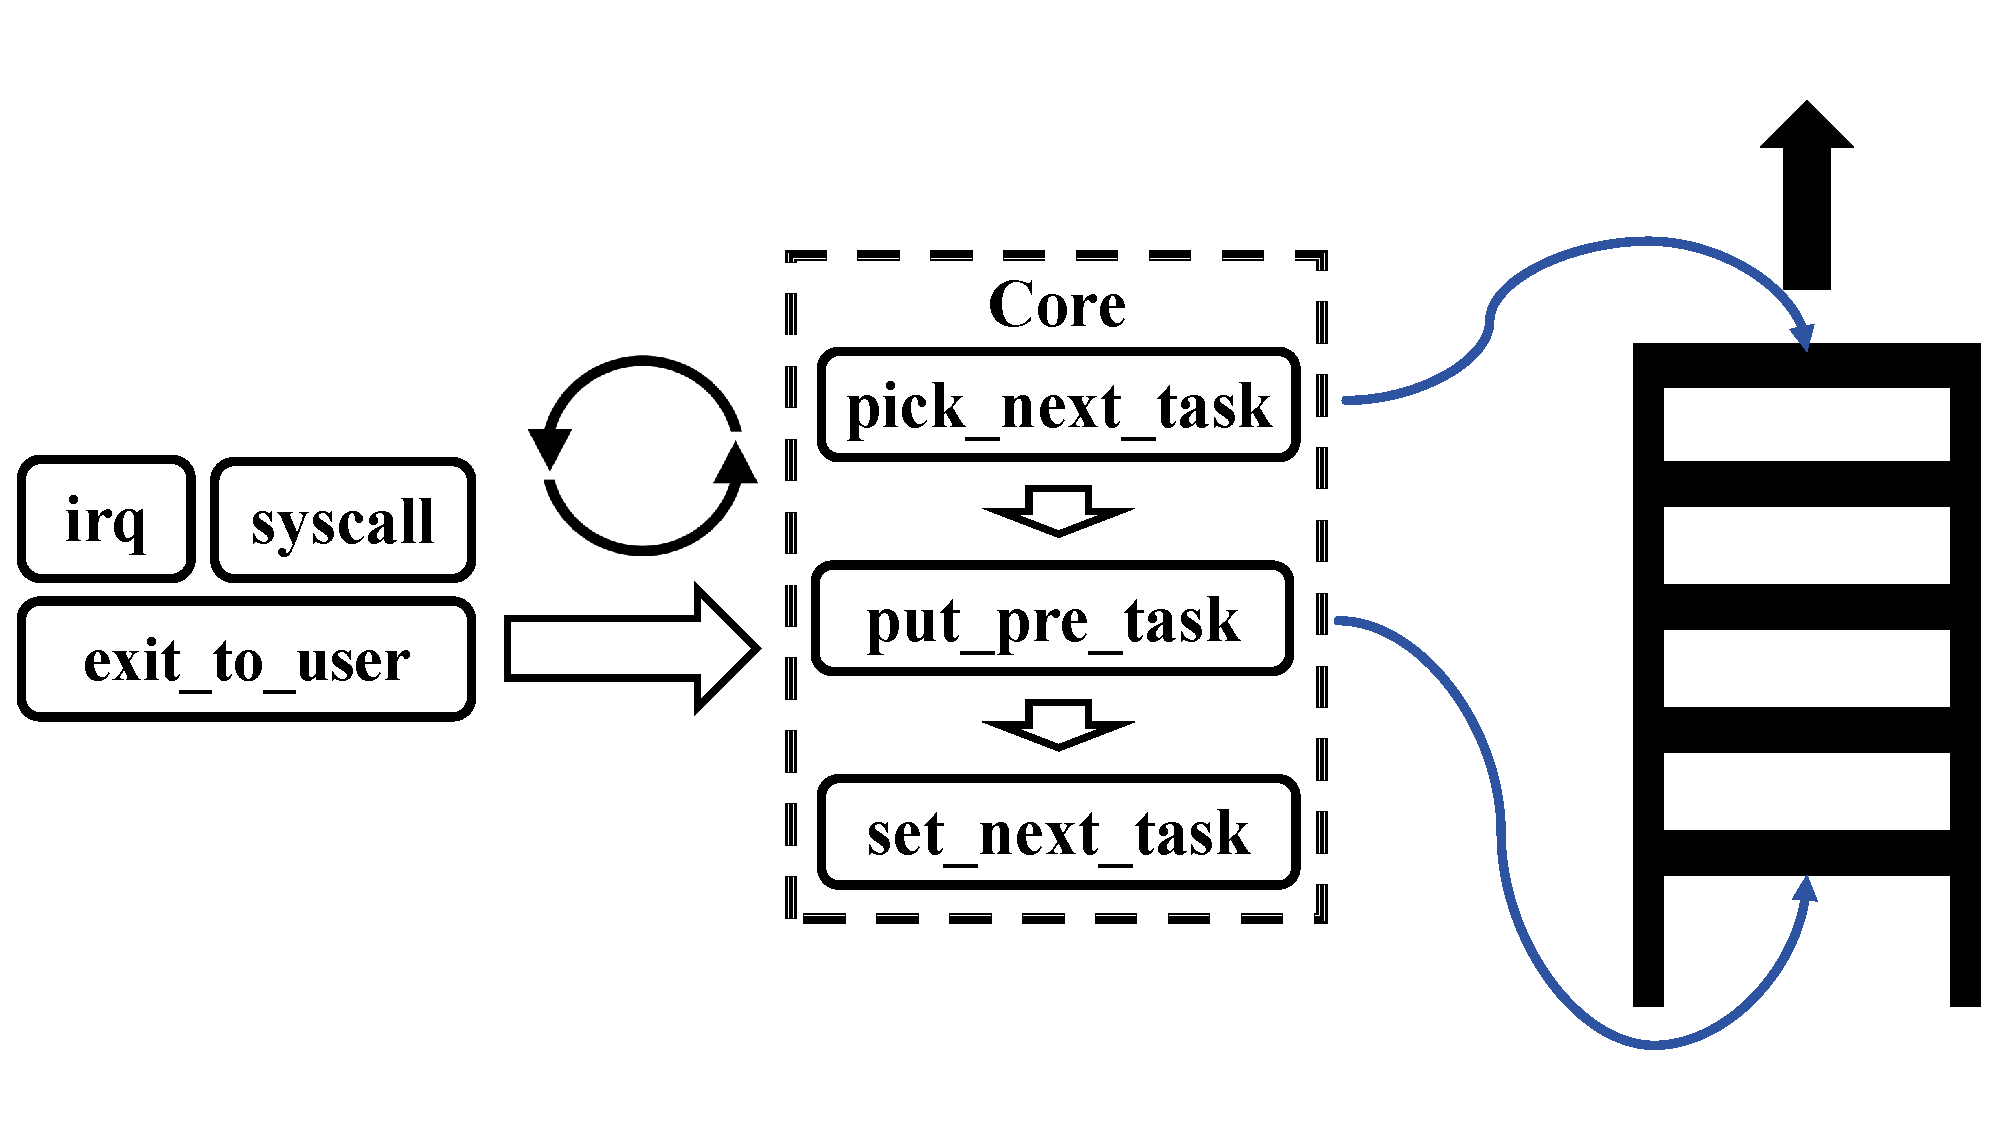
\includegraphics[width=0.6\textwidth]{shcedule_loop}
    \bicaption{\quad 调度循环}{\quad Scheduling loop}
    \label{fig:shcedule_loop}
\end{figure}

    \item Sched Policy调度策略层基于调度类层,并提供优先级机制的实现。不同调度策略的优先级机制的实现各不相同。FIFO调度策略提供了多个优先级队列,并保证高优先级队列中的任务总被优先调度。RR调度策略中所有任务按时间片轮流执行,当一个时间片结束时,调度器会检查Run Queue上的所有任务,并选择优先级最高的进行执行。NORMAL与BATCH调度策略中的优先级决定了vruntime的积累速度,而在Fair调度类中任务的vruntime越小则获得调度的概率越高。

\end{itemize}

\section{BPF技术}

% 定制内核的需求: 多样的硬件/多样的网络处理模式
% 内核模块: 灵活性高,但不安全,容易引发内核crash风险
% BPF在网络子系统引入,自定义网络包的处理流程
% 逐渐拓展到各个子系统中,但由于内核的审慎地设计,其他子系统中通常用来进行只读操作,如进行监测

eBPF(Extended Berkeley Packet Filter)是一个运行在Linux内核中的轻量、高效64位的类RISC虚拟机\citep{sharaf2022extended}。eBPF凭借其强大的性能,及在可移植性、灵活性与安全性的优势,得到了工业界和学术界的广泛认可,并逐渐成为在内核中执行不可信的、用户定义的专用代码的最佳实践和事实标准。

eBPF的前身是BPF(Berkeley Packet Filter),由McCannel和Jacobson提出\citep{mccanne1993bsd},用于在Linux网络子系统中自定义网络包的处理。BPF优异的设计与理念得到了Linux社区贡献者的广泛认可,并逐渐扩展到除网络子系统以外的其他子系统中。为进行区分,Linux社区将早期的BPF技术称为cBPF(Classic Berkeley Packet Filter)。当前BPF与eBPF均指代最新的BPF技术,本文后续说明中也使用此做法。

BPF虚拟机包含10个通用寄存器以及1个只读的帧指针寄存器,位宽均为64-bits。与JVM类似,BPF虚拟机采用字节码作为执行指令的格式,并定义了一套完整的指令集。BPF字节码作为一种中间语言,解耦了编译环境与执行环境,实现可移植性的同时保证了运行性能。同时,BPF字节码相较于机器码语义更清晰,使得内核能够更好进行验证来减少风险代码。

cBPF程序仅支持BPF汇编编写,而当前随GCC、Clang等主流编译器对BPF字节码的支持,开发者可使用C、Rust等高级语言开发BPF程序\citep{ebpfguidence}。然而BPF程序并非是图灵完备的,因此仅能使用高级语言的子集进行开发。编译好的BPF程序是常规的ELF文件,并由内核态的BPF虚拟机执行。BPF程序的加载运行依赖一系列系统调用完成。在加载BPF程序的系统调用中,内核首先会尝试运行BPF程序,并验证其中的未定义行为,如越界的内存访问、不确定的循环等。对合法的BPF程序,内核会将其保存到专门的内存区域,并附加到指定的内核插桩点。此后,每次到达插桩点时,内核就会跳转至BPF虚拟机并解释执行附加的BPF程序。

BPF技术通常会与同样作为内核功能扩展的内核模块比较,而相较于内核模块,BPF技术的优势体现在更高的安全性上,主要体现在两个方面:

\begin{enumerate}
    \item BPF程序的编写限制更严格。一方面,BPF并非图灵完备的,因此程序逻辑通常较为简单,并一定程度上减少未定义行为的出现。另一方面,Linux内核会在BPF程序加载时进行验证,并拒绝加载非法的BPF程序,从而避免执行不安全的代码。
    \item BPF程序与内核的交互更受控。内核模块与内核的交互通过直接的函数与变量访问实现,而不做限制的交互模式存在较大的安全风险。相反,BPF程序仅允许通过BPF Helper函数来与内核交互,包括对内核数据的读写、共享内存使用等。BPF Helper函数限制了BPF程序所能访问的内核功能,以达到受控的交互。其次,部分BPF Helper函数保证线程安全,提供基本的安全性保证。最后,BPF程序所能附着的插桩位点由内核提供,因此BPF程序的影响范围也是受内核控制的。
\end{enumerate}

\begin{figure}[!htbp]
    \centering
    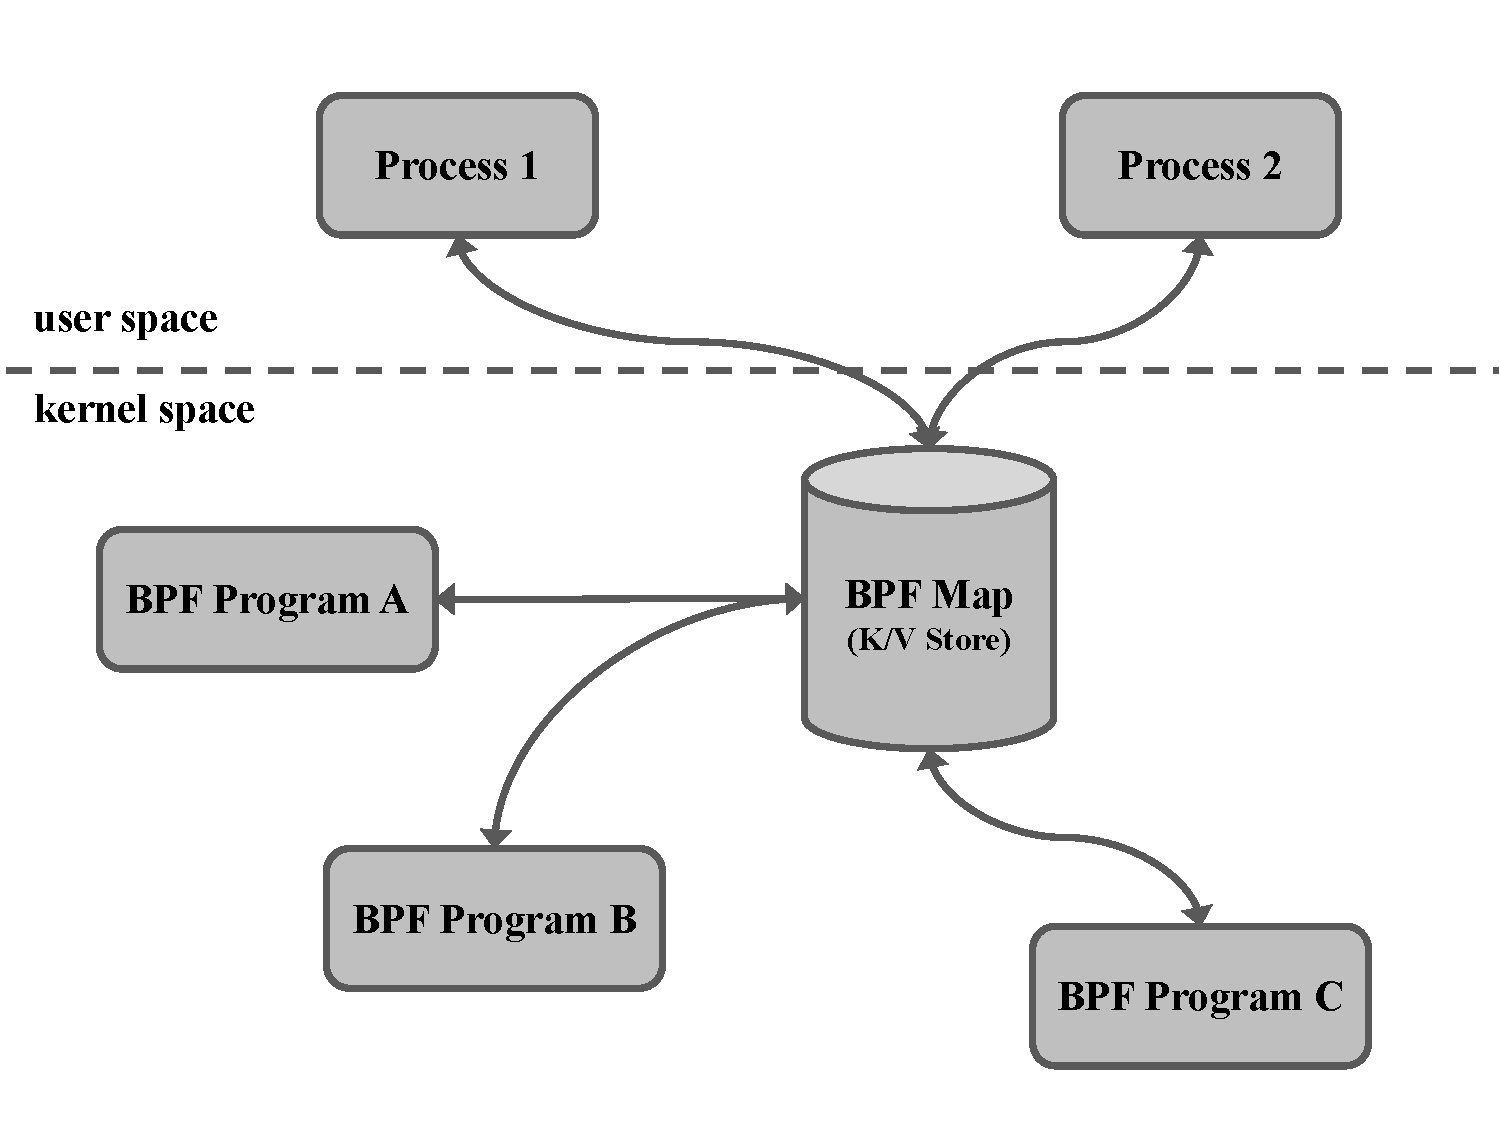
\includegraphics[width=0.5\textwidth]{bpf_user_kernel}
    \bicaption{\quad BPF程序中的用户态与内核态的交互}{\quad Interaction between user space and kernel space in BPF programs}
    \label{fig:bpf_user_kernel}
\end{figure}

BPF技术具有高度的灵活性。首先,开发者可利用libbpf等库来对BPF程序文件进行操作,如读写BPF程序中的全局变量、选择性地加载部分BPF程序等。其次,开发者可通过如图~\ref{fig:bpf_user_kernel}所示的BPF Map实现BPF程序之间、BPF程序与用户态程序间的共享内存。一方面,用户程序可通过BPF Map来安全地读写内核数据,如读取BPF程序采集的信息或者修改BPF程序的行为。另一方面,BPF程序之间可通过BPF Map传递数据以实现彼此间的合作。最后,开发者可在BPF程序间进行如图~\ref{fig:bpf_to_bpf}所示的相互调用,从而突破内核对单个BPF函数的限制,实现更复杂的逻辑。

\begin{figure}[!htbp]
    \centering
    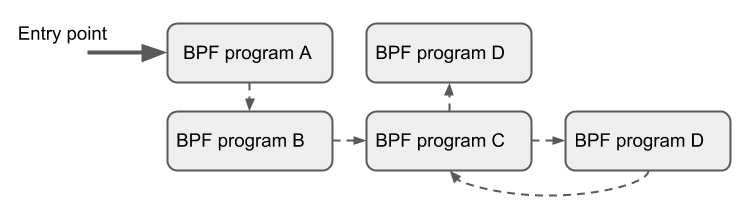
\includegraphics[width=0.7\textwidth]{bpf_to_bpf}
    \bicaption{\quad BPF程序之间的相互调用}{\quad Invocation between BPF programs}
    \label{fig:bpf_to_bpf}
\end{figure}

BPF程序通常在加载后由BPF虚拟机解释执行,这种低效方式会对内核性能产生一定的影响。为提升BPF程序的执行效率,Linux内核提供了BPF JIT配置选项,允许BPF程序在加载时直接编译为本机机器码,并替换原BPF程序。此后,插桩点触发时不再由BPF虚拟机解释执行,而是在捕获到内核栈上数据后就直接跳转到BPF程序处执行。BPF JIT配置在保持BPF程序移植性的同时,大大提高了BPF程序的执行效率。

BPF技术也存在一些不足。首先,BPF程序并非图灵完备且在栈空间上有严格的要求,尽管保证了一定的安全性,但也因此无法实现较大规模的程序。其次,BPF运行在内核环境中,依赖BPF Helper函数来与内核交互,而当前内核仅在有限的子系统中开放了交互功能。不过BPF技术在灵活性与安全性上的优势得到了内核开发者以及云原生社区的重视。当前Linux内核社区中的BPF-next SIG致力于解决BPF技术的种种问题,并尝试逐步增强BPF程序的功能以便于向更多子系统推广。

BPF技术开源社区维护十分积极,当前主流生态可分为BCC(BPF Compiler Collection)\citep{bcc}与libbpf\citep{libbpf}两支:

\begin{enumerate}

    \item BCC提供了基于Pyhton语言的元编程框架。BCC包含了完整的BPF编译环境,并在运行时自动识别目标机器的内核来进行BPF程序编译和加载。开发者只需要定义少量的BPF程序文本,完整的BPF代码生成、内核兼容性、编译环境选择均由BCC完成。元编程框架大大降低了BPF程序的开发难度,在目标机器上进行编译也有利于解决内核版本兼容性问题。但这种方式不仅引入了额外的编译环境开销,同时编程框架的过度封装也不利于快速使用新的BPF特性。

    \item libbpf采用CO-RE(Compile Once – Run Everywhere)的思想。CO-RE即在本地将BPF编译为字节码并保存为只读数据。开发者可通过libbpf提供一系列辅助函数读写编译好的BPF程序,并利用库函数完成BPF程序的加载、附加及卸载。相较于BCC,使用libbpf能够减少存储空间的占用,同时由于不需要在目标机器上编译,能够做到更快速地部署。为解决内核版本的兼容性问题,开发者可使用bpftool工具来生成目标内核版本的符号信息,并编译适用目标内核的BPF程序。此外,开发者也可在BPF程序中声明内核版本兼容性,避免不兼容版本内核的加载。

\end{enumerate}

\section{可扩展调度类}

Sched Ext可扩展调度类项目\citep{schedext},由Meta工程师在2022年提出,用来满足Meta数据中心对内核调度策略定制的需求。Sched Ext项目的整体架构如图~\ref{fig:sched_ext_arch}所示,主要包含两个部分:Ext调度类和调度器开发工具。其中Ext调度类包含一系列补丁集,由Meta工程师与内核社区工作者共同维护。调度器开发工具提供了C与Rust语言的开发库支持,协助对BPF程序的管理及用户态调度器的开发。Sched Ext项目当前已在Meta集群中部署与测试,且项目社区十分活跃。

\begin{figure}[!htbp]
    \centering
    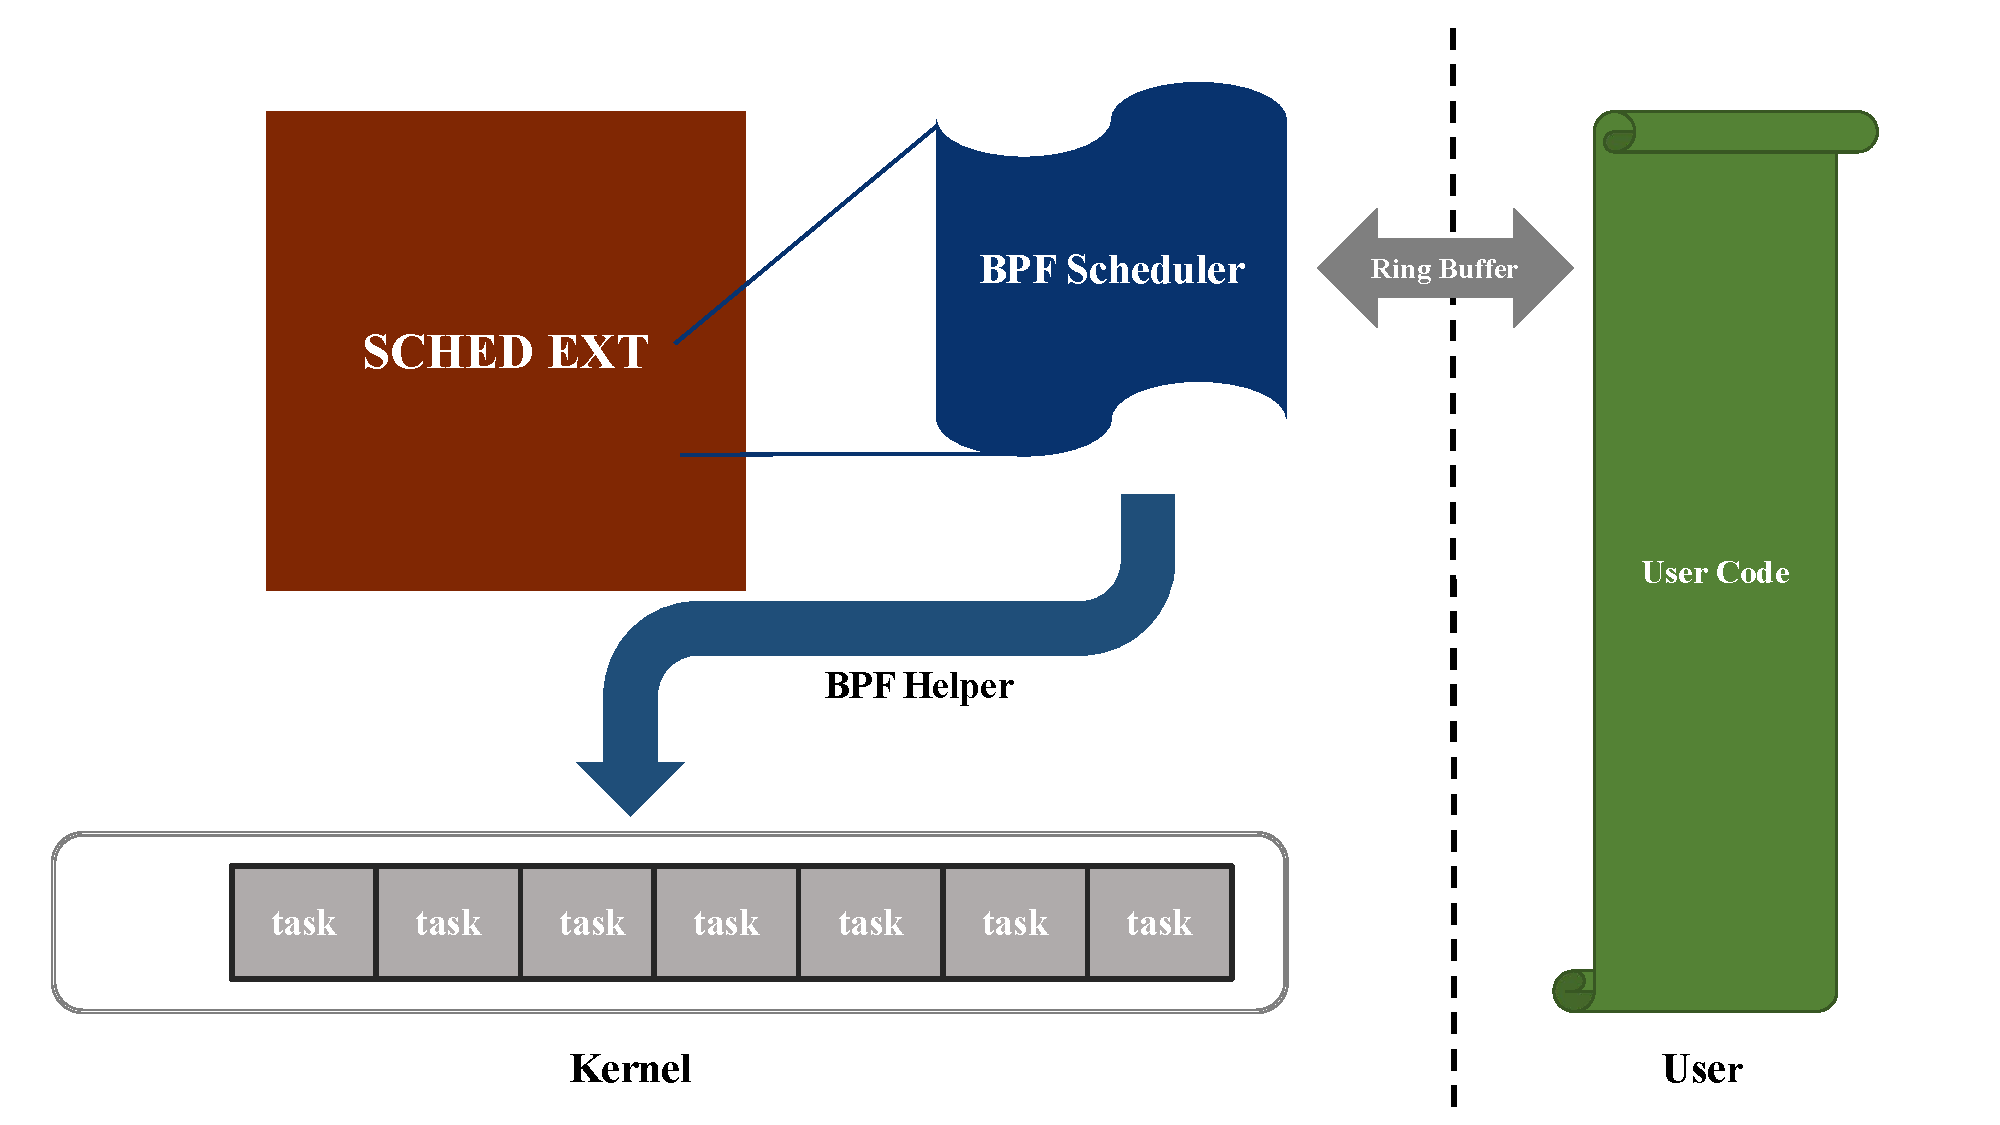
\includegraphics[width=0.65\textwidth]{sched_ext_arch}
    \bicaption{\quad Sched Ext项目架构}{\quad Architecture of the Sched Ext project}
    \label{fig:sched_ext_arch}
\end{figure}

Sched Ext项目启发自ghOSt\citep{humphries2021ghost},通过插件化的内核调度类来提升Linux内核调度子系统的灵活性。Sched Ext项目使用BPF技术作为调度子系统可扩展性的实现。一方面由于BPF程序运行在内核态,相较于使用系统调用的ghOSt运行效率更高。另一方面,BPF技术提供了丰富的与用户态程序、其他BPF程序交互的手段,支持更灵活调度策略的设计。不同于ghOSt,Sched Ext项目在设计时就尽可能保持与现有调度子系统的兼容性。如图~\ref{fig:sched_ext_priorty}所示,Sched Ext项目新增了Ext调度类,并将优先级设置在Fair调度类与Idle调度类之间。同时,即使设置任务的调度类为Ext,在没有BPF程序加载时,任务仍会按Fair调度类的逻辑进行调度。以上都保证了对于现有调度子系统最小的影响。 

\begin{figure}[!htbp]
    \centering
    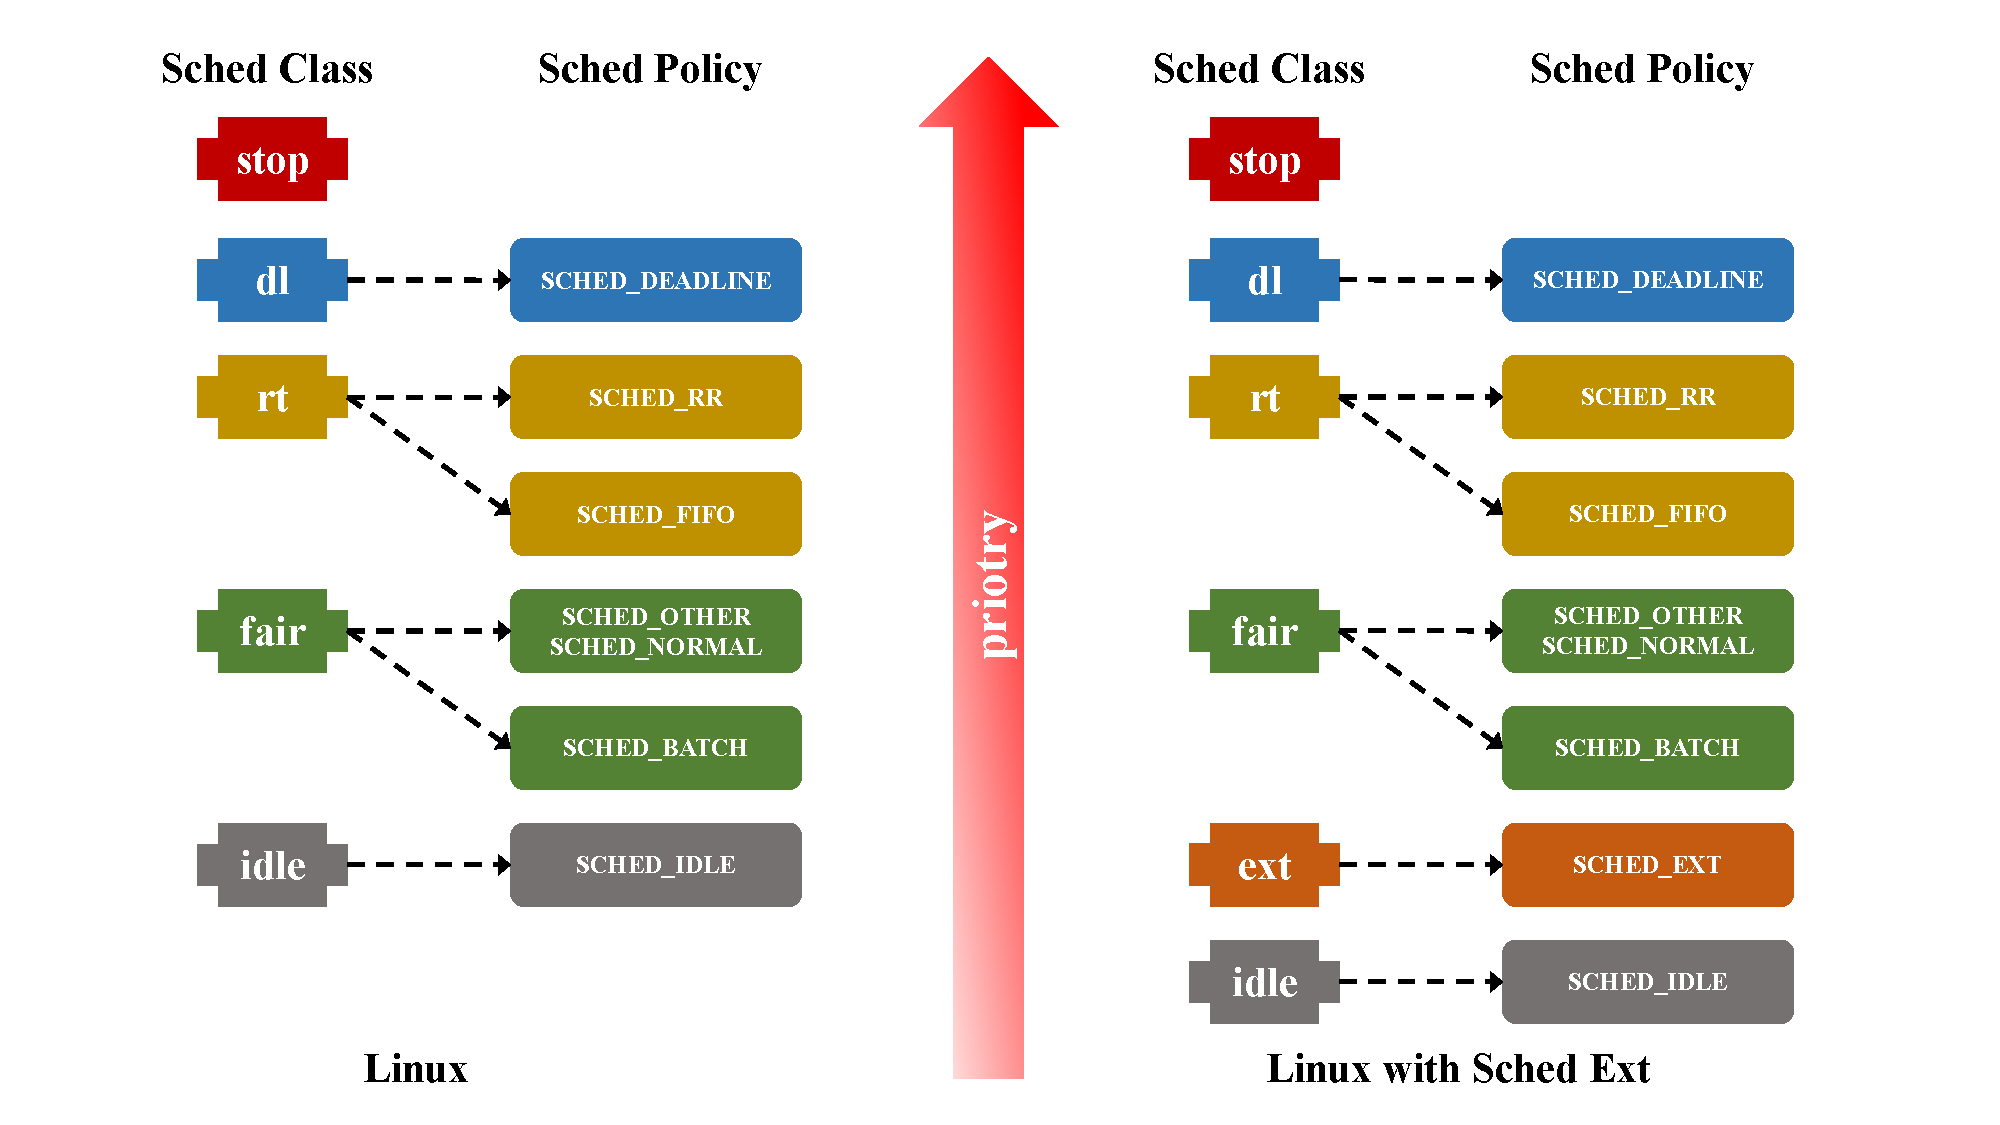
\includegraphics[width=0.75\textwidth]{sched_ext_priorty}
    \bicaption{\quad Ext调度类优先级}{\quad Priority of the Ext scheduling class}
    \label{fig:sched_ext_priorty}
\end{figure}

Sched Ext项目提供了一种使用BPF程序定制调度策略的方式,实现这一目标依赖DSQ(Dispatch Queue)与一系列BPF Helper函数。DSQ用于在Ext调度类和BPF程序之间共享任务队列。初始化时,Ext调度类会为每个CPU创建一个Local DSQ。而在运行过程中,Ext调度类管理的每个CPU都会尝试从Local DSQ中获取任务。此外,BPF程序也可创建独立的数个DSQ来支持复杂调度策略的设计。Sched Ext项目提供了额外的BPF Helper函数,用来进行DSQ的管理及与Ext调度类的交互,具体BPF Helper函数的作用如下:

\begin{itemize}

    \item \textbf{scx\_bpf\_create\_dsq}: 定义DSQ来对任务进行管理。BPF程序可创建数个DSQ,每个DSQ都有自己的独立ID。同时允许指定DSQ所在的NUMA node以实现更高的内存访问效率。

    \item \textbf{scx\_bpf\_dispatch、scx\_bpf\_dispatch\_vtime}:调度任务到指定的DSQ中。BPF程序可指定DSQ ID来将任务调度到DSQ上。同时,BPF程序可为任务设置此次调度的时间片大小。时间片的特殊值SCX\_SLICE\_INF会让任务保持运行直到结束或主动释放。DSQ默认使用FIFO策略来管理任务的出入队,Sched Ext还提供了vtime DSQ,能够实现类CFS的任务管理。

    \begin{figure}[!htbp]
        \centering
        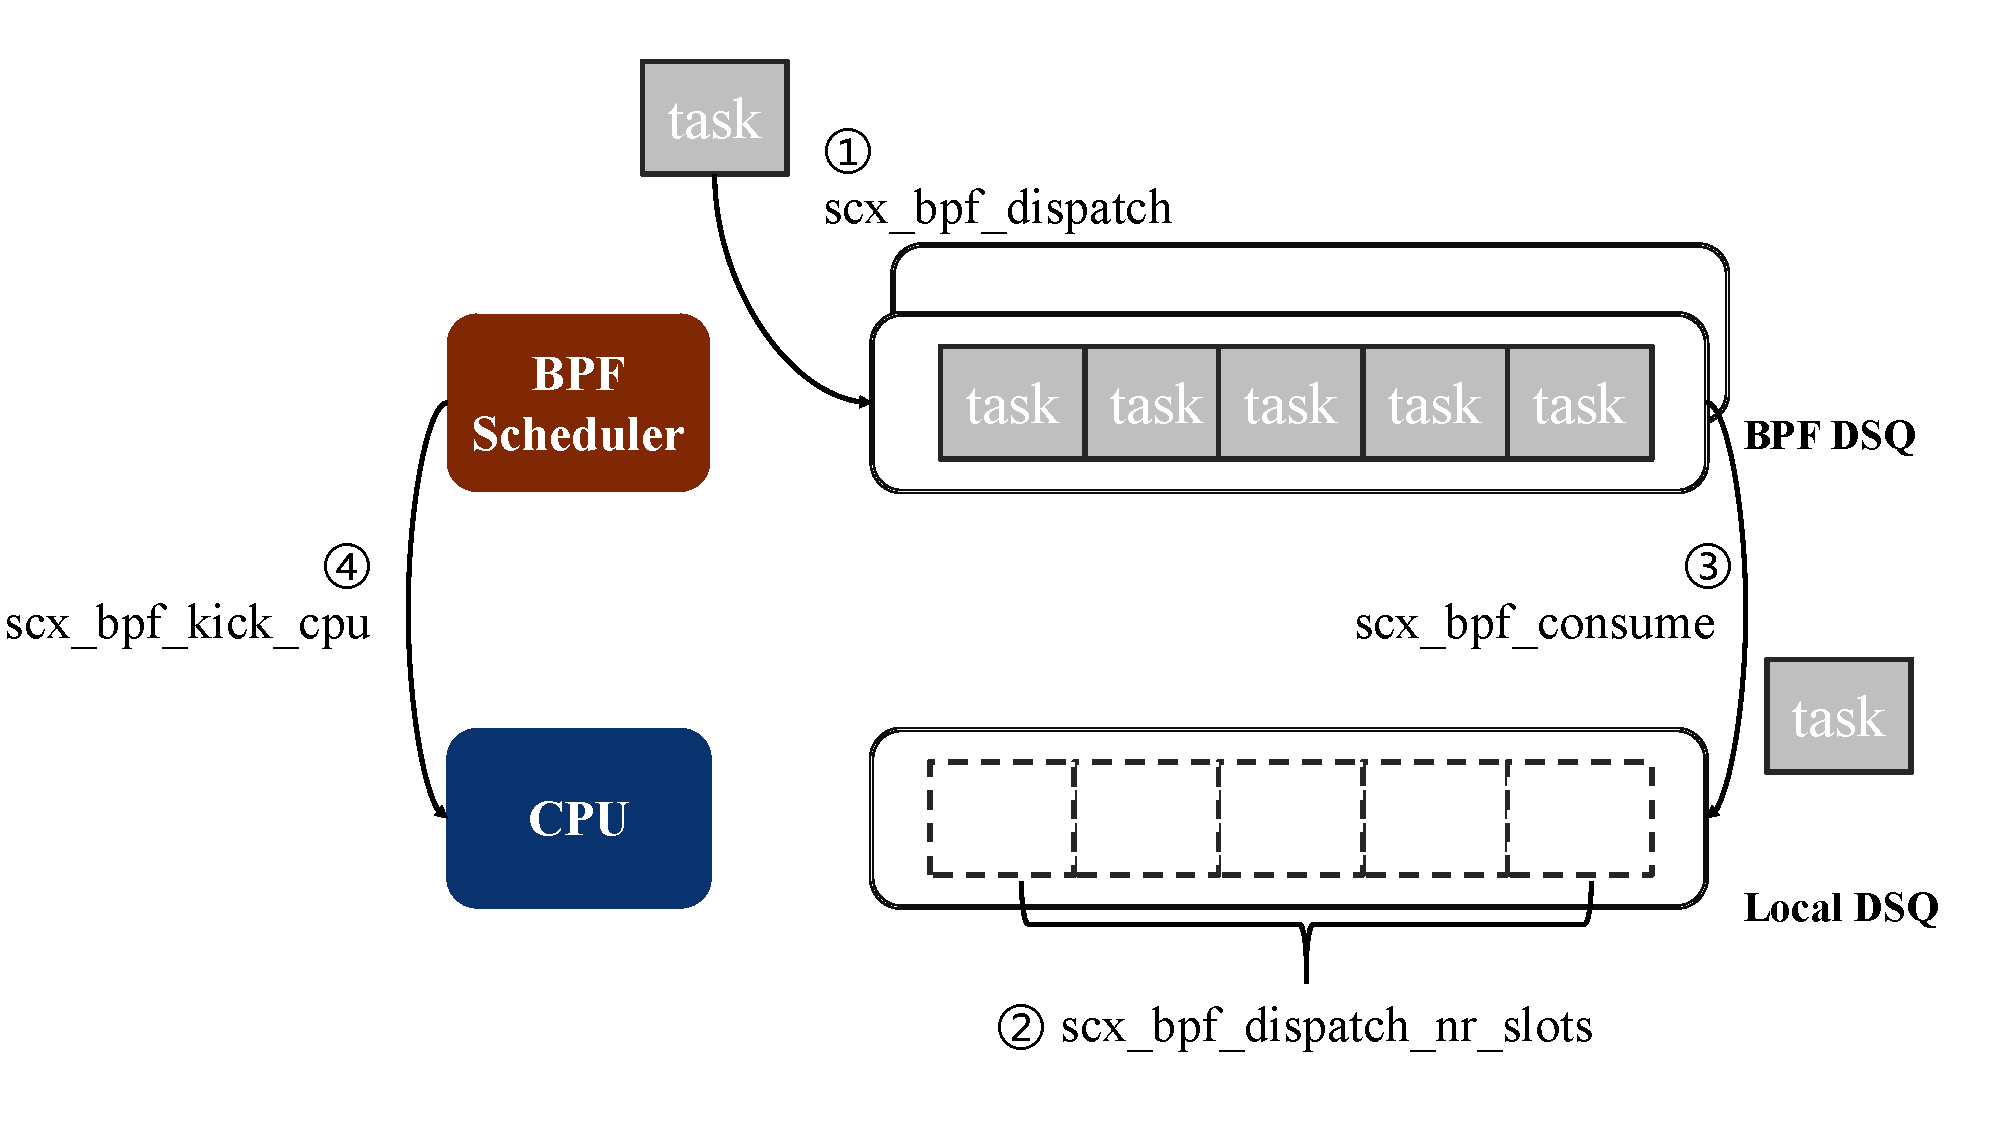
\includegraphics[width=0.8\textwidth]{sched_ext_helpers}
        \bicaption{\quad Sched Ext中的BPF Helper函数}{\quad BPF helper functions in Sched Ext}
        \label{fig:sched_ext_helpers}
    \end{figure}
    
    \item \textbf{scx\_bpf\_dispatch\_nr\_slots}:查看CPU可调度的任务槽数。BPF程序在调度任务前可检查目标CPU Local DSQ上的空余任务槽位的数量,避免向目标CPU调度过多的任务。

    \item \textbf{scx\_bpf\_dispatch\_cancel}:撤销最近调度的一个任务。BPF程序可撤销向DSQ上最近调度的任务,重复执行此操作可撤回更多的任务。BPF程序中可以定义多个DSQ,回撤手段便于管理已调度的任务。
    
    \item \textbf{scx\_bpf\_consume}:从其他DSQ调度一个任务到当前CPU上。在DSQ之间迁移任务需要考虑并发问题,此Helper函数则提供了方便的封装,BPF程序可便捷地将其他DSQ中的任务调度到当前CPU上。

    \item \textbf{scx\_bpf\_kick\_cpu}:唤醒目标CPU。BPF程序可向目标CPU发送IPI。IPI会唤起目标CPU上调度循环的执行,从而唤醒Idle CPU或进行抢占。BPF程序可在此Helper函数上等待,期间会重复执行低功耗指令并保持CPU的占用。

    \item \textbf{scx\_bpf\_pick\_idle\_cpu}:寻找空闲的CPU。BPF程序可获取一个空闲CPU的ID。Ext调度类会追踪CPU的状态,并记录空闲的CPU。依据不同的调度目标,BPF程序可以将任务分发到不同的CPU中,而通过此Helper函数BPF程序能够较方便地找到空闲CPU。

\end{itemize}

Ext调度类还提供了一系列插桩位点,便于BPF程序参与到调度决策过程中。以调度循环为例,Ext调度类通过如图~\ref{fig:ext_bpf}所示的流程来与BPF程序协作完成调度过程。其中,Ext调度类会在核心逻辑的关键点处唤起BPF程序执行,并将BPF程序的返回结果作为决策依据之一。Sched Ext项目中将这些插桩点抽象为sched\_ext\_ops函数集合,BPF程序可以实现其中的部分或全部的函数,每个函数的插桩点与具体作用为:

\begin{figure}[!htbp]
    \centering
    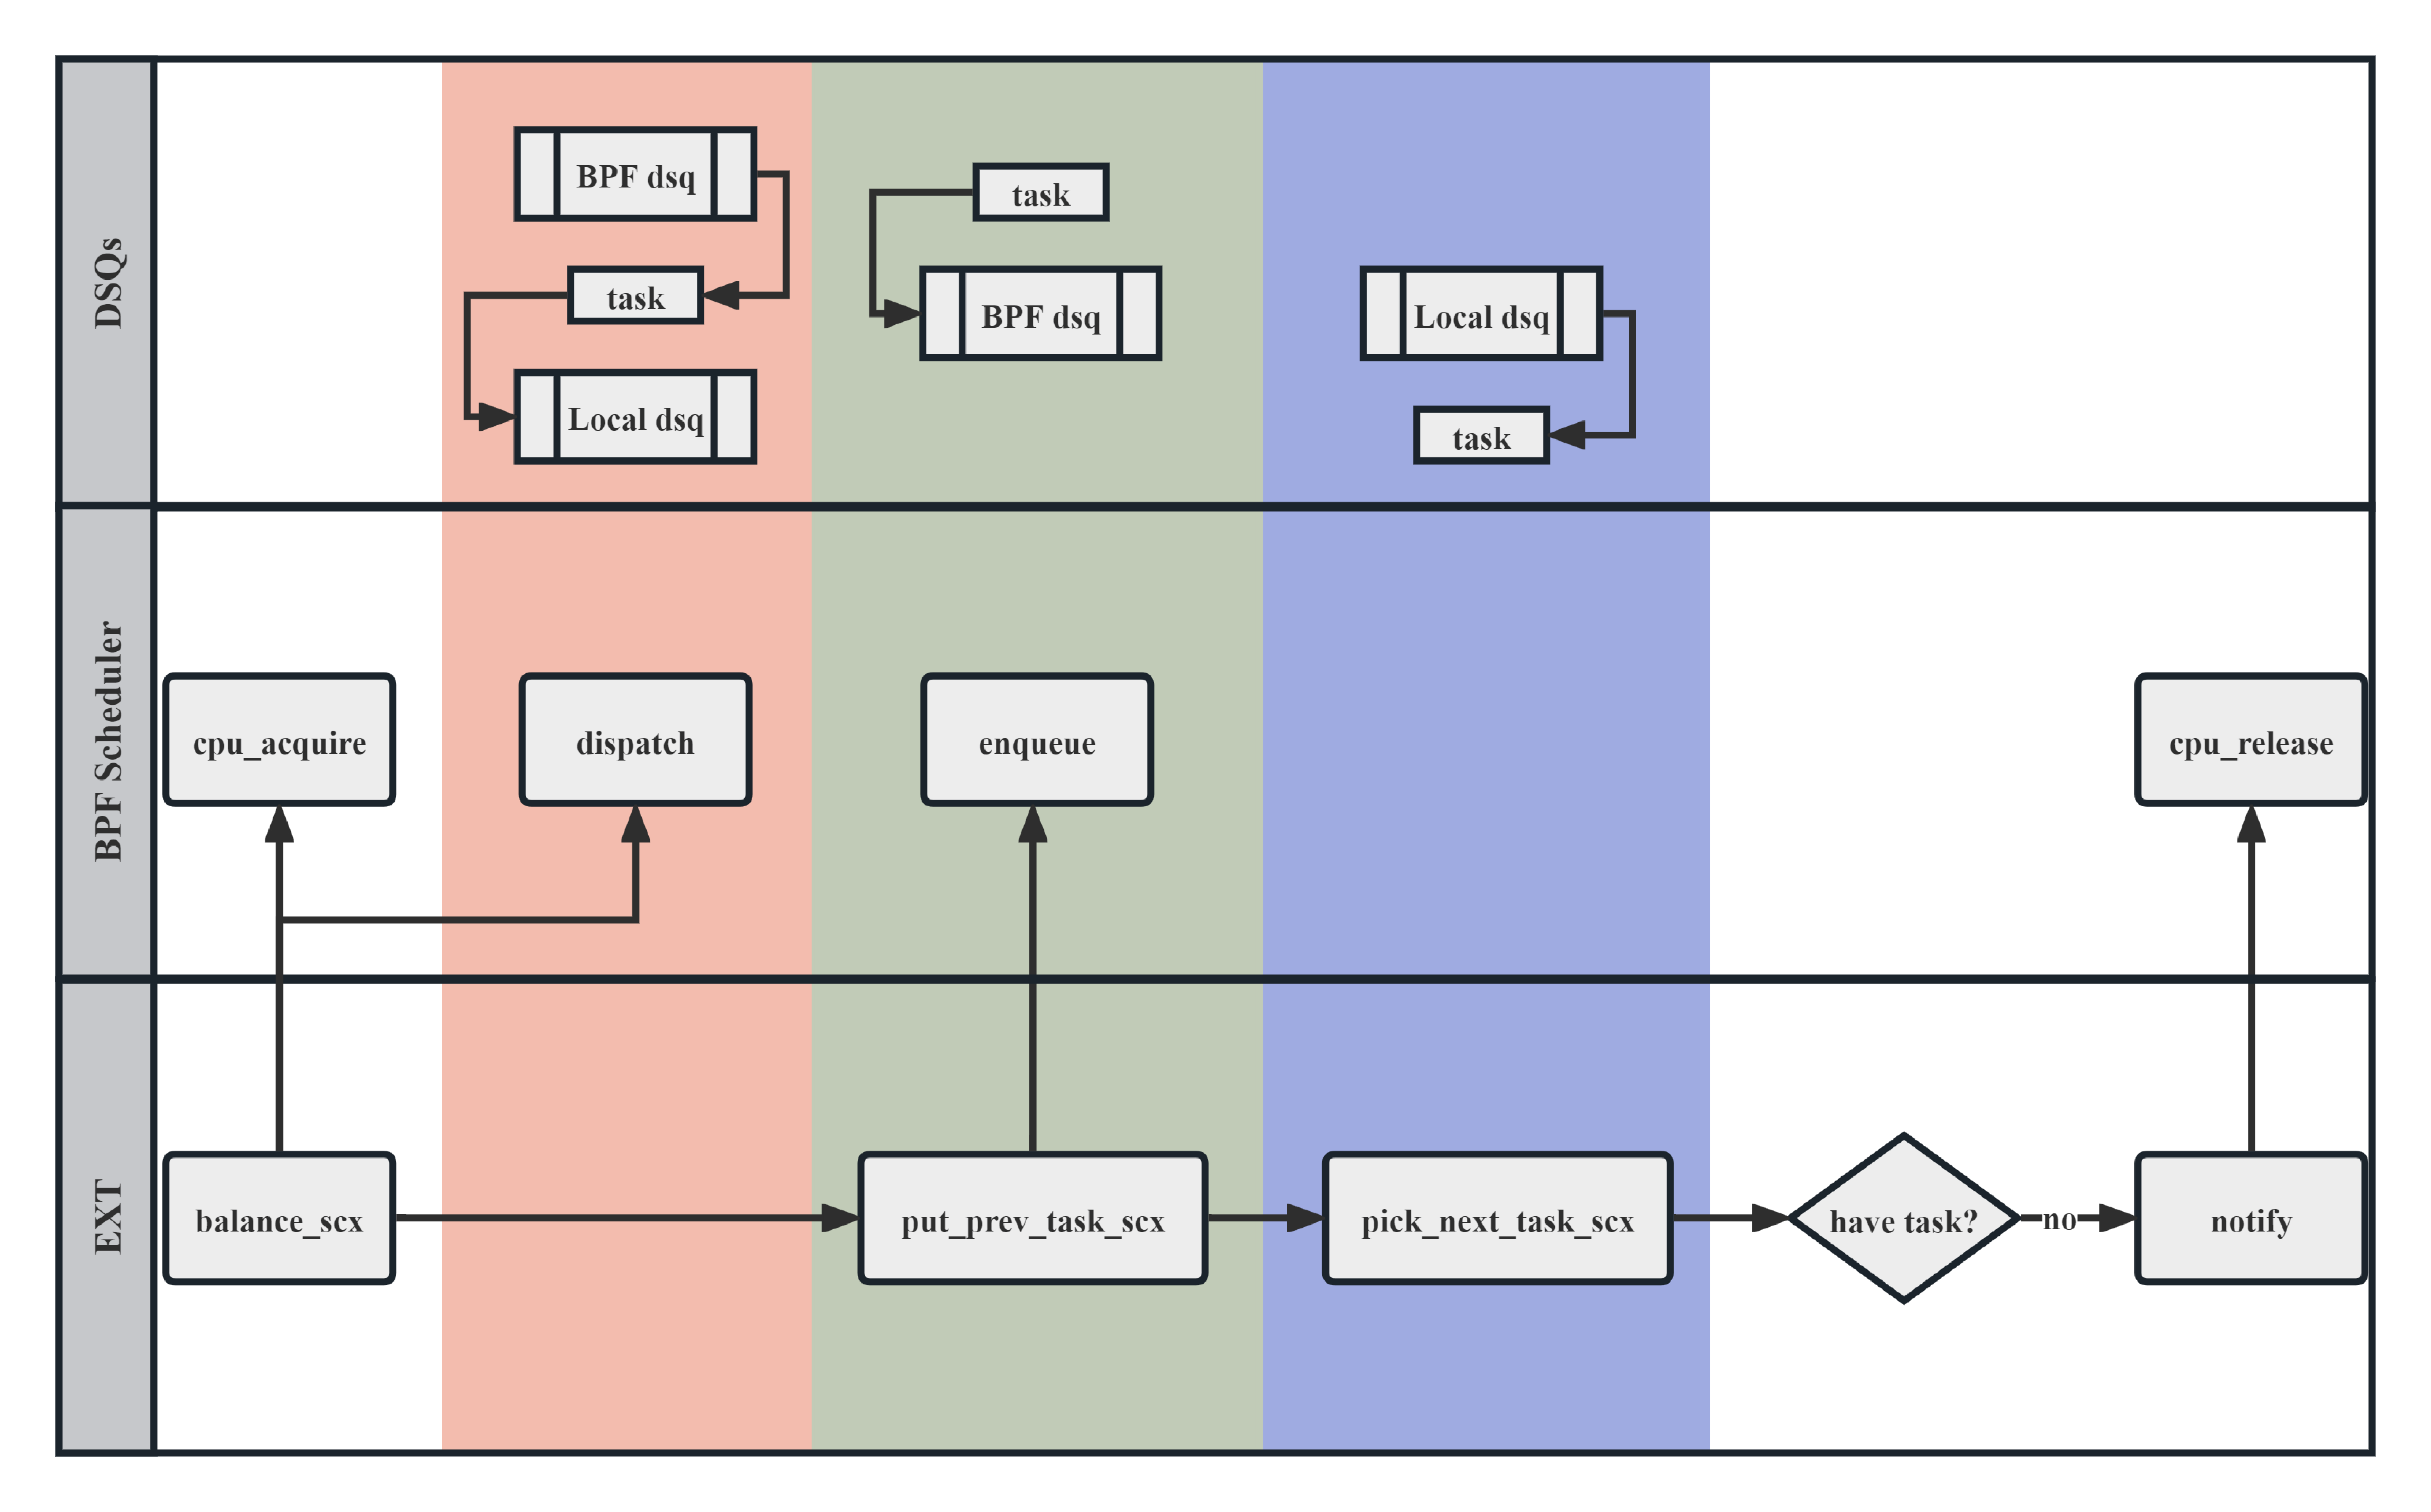
\includegraphics[width=0.95\textwidth]{ext_bpf}
    \bicaption{\quad Ext调度类与BPF程序协作进行调度循环}{\quad 
    Ext schedule scheduling collaborating with BPF programs for scheduling loop}
    \label{fig:ext_bpf}
\end{figure}

\begin{itemize}

    \item \textbf{select\_cpu}:Ext调度类选择CPU过程的位点。BPF程序可为唤醒的任务选择一个CPU,需要考虑任务的特性以及CPU的负载情况。CPU的选择结果会影响到系统总体的性能,
    因此Ext调度类还会结合其他信息来CPU选择的决策。

    \item \textbf{enqueue}:Ext调度类处理任务的入队过程的位点。Ext调度类管理的任务就绪时,会唤起此BPF程序的执行。BPF程序可以为此任务选择一个CPU,或者将其加入自定义的DSQ中来管理。

    \item \textbf{dequeue}:Ext调度类处理任务的出队过程的位点。修改任务的调度参数,如静态优先级时,会触发Ext调度类的出队逻辑,并唤起此BPF程序的执行。BPF程序可以通过捕获传入的参数,并结合已有的数据来定制优先级机制的实现。
    
    \item \textbf{dispatch}:Ext调度类处理任务调度过程的位点。Ext调度类中每个CPU都有自己的Local DSQ,同时BPF程序也可以创建数个DSQ。当CPU发现Local DSQ为空时,就会触发此BHPF程序。BPF程序可调度一个或数个任务到CPU的Local DSQ中,也可以不进行调度。当BPF程序没有返回有效的任务时,Ext调度类便会放弃CPU的管理权。
    
    \item \textbf{tick}:Ext调度类处理任务滴答过程的位点。Ext调度类在处理任务滴答时,会唤起此BPF程序的执行。BPF程序可以获取滴答时正在执行的任务,并自定义滴答逻辑,如更新时间记账信息、遍历DSQ等。同时,BPF程序可将任务的时间片设置为0,使得在回到Ext调度类时立刻触发一次dispatch操作。

    \item \textbf{runnable、running、stopping、quiescent}:Ext调度类追踪任务状态的过程中。任务通常会在如下三种情况进入Runnable状态:被唤醒、回到调度队列、从其他CPU迁入时,如任务从等待IO状态中恢复、完成静态优先级的修改时,都会进入Runnable状态,并唤起BPF程序的执行。其余位点原理类似,其中quiescent状态转化与runnable相反,running对应任务将要在CPU上调度时,而stopping对应任务将要从CPU上换下时。BPF程序通过感知任务状态的变换,能够实现自定义的处理逻辑。
    
    \item \textbf{yield}:Ext调度类处理任务出让CPU资源过程的位点。对于多线程,Linux提供了sched\_yield系统调用来允许任务主动放弃CPU资源。线程的退出之后依赖调度器来选择下一个任务。Ext调度类会唤起BPF程序的执行,BPF程序可定制下一个任务的选择逻辑。

    \item \textbf{cpu\_acquire、cpu\_release}:Ext调度类追踪CPU占用情况过程的位点。Ext调度类获取CPU管理权时,会触发cpu\_acquire处BPF程序的执行,反之则触发cpu\_release处BPF程序的执行。CPU管理权变化通常意味着更高优先级的调度类没有要执行的任务,或当前调度类没有要执行的任务。BPF程序可通过这两个位点来追踪Ext调度类能够管理的CPU。

    \item \textbf{init\_task、exit\_task}:Ext调度类追踪任务的创建与退出过程的位点。Ext调度类在任务的创建与退出时会唤起对应BPF程序的执行。BPF程序可在这些位点处为每个任务单独创建额外的追踪信息,并在任务结束时进行销毁。

\end{itemize}

\section{沙箱技术}

% 系统级沙箱(虚拟机),容器级沙箱(进程)
% 安全性: 虚拟机 > 沙箱
% - 容器类沙箱缺乏调度机制的支持,而对调度机制的修改需要更安全的沙箱环境来限制风险的传播

沙箱技术是一种安全机制,用于提供隔离的运行环境,以便在受限的环境中执行不受信任的程序。沙箱技术能够隔离程序所能使用的资源,如CPU、内存、网络等,并防止这些程序影响主机上其他程序。沙箱技术提供了安全运程序的基础,数据中心中常见的沙箱技术包括虚拟机技术与容器技术。

虚拟机技术是数据中心使用广泛的沙箱技术。虚拟机指通过软硬件的手段在已运行的系统中模拟出一个硬件环境,并能够支持运行其他系统。虚拟机概念可追溯到VM/370\citep{creasy1981origin}时代,而后Mendel Rosenblum提出了Disco\citep{bugnion1997disco}用来解决操作系统迭代速度与硬件更新速度不匹配的问题。其中依托虚拟设备与虚拟机环境来提升操作系统的迭代速度这一理念,指明了后续虚拟机发展的方向。而随着虚拟化技术的不断发展,虚拟化开销也逐渐降低。软件上从运行在裸金属上的Type 1虚拟化技术Xen\citep{barham2003xen},到能够将Linux转化为一个Hyeprvisor的Type 2虚拟化技术KVM\citep{kivity2007kvm},虚拟化软件技术的不断发展使得虚拟机的管理越来越简单。硬件上基于SRIOV的设备直通手段\citep{dong2012high},让虚拟机能够直接接触物理设备,从而达到几乎与裸金属操作系统相近的性能。虚拟机具备较高的隔离性,能够较好的处理多租户场景下的安全性问题,以上这些为虚拟机在云厂商中较长时间的广泛使用提供了基础。

容器技术期望提供一种进程级别的沙箱,来隔离运行在同一系统上的不同进程。程序的执行依赖一定的运行环境,Linux早期的发展过程中,由于包管理工具的不成熟,不同程序之间会相互污染运行环境,造成程序的运行错误或失败。为解决此问题,Linux提供了chroot工具以及相关的系统调用,允许为程序设置不同的根目录。让不同的程序运行在满足各自运行环境的根目录中,解决了程序相互之间的依赖污染问题。chroot实质是一种文件系统的隔离机制,而后在Linux的不断发展过程中,各个子系统的隔离机制都被实现。其中Cgroup与Namespace机制构成了现代容器技术的基础。Namespace技术提供了Mount、UTS、IPC、PID、Network及User等系统资源的隔离,使得容器中的进程认为自己运行在一个独立的系统环境中。Cgroup技术则提供了CPU、Memory、BlkIO、NetIO、Devices等硬件资源的隔离,使得容器中的进程能够运行在一个受限制的硬件资源环境中。OverlayFS(Overlay File System)技术能够将多层文件目录叠加为一个独立的文件目录,同时允许各层之间有独立的读写行为,并借助COW(写时复制)来解决各层文件共享的问题。OverlayFS技术为容器镜像技术提供了基础,而借助标准化的OCI镜像,容器得以方便地在不同的发行版、软件环境的Linux系统中传播。容器的易用性催生了容器编排技术,而以Kubernetes为主的容器编排技术在数据中心中发挥越来越大的作用。

容器在本质上仍然是进程,在执行效率上高于虚拟机。但由于进程共享了相同的内核,因而不可避免地保有进程的安全问题,而这点在多租户场景的云环境中尤为重要。现代容器技术提供了各种各样的手段提升容器的安全性,如限制容器中进程能够使用的系统调用等,然而这种方式牺牲了容器的通用性,容易导致部分容器的运行异常。安全容器的提出就试图解决这一问题,安全容器本质上是一个高度裁剪的虚拟机,运行着一个同样高度裁剪的内核。这些做法大大精简了虚拟化环境并减少开销,使得虚拟机启动速度提升的同时,减少虚拟机本身的内存占用。同时,多数容器镜像都包含了一个完整的根文件系统,因能够稍作处理后作为一个虚拟机镜像使用。安全容器作为一种沙箱技术,结合了虚拟机的强隔离性与容器的易用性。其中在虚拟机监视器上,阿里的RunD\citep{li2022rund}、AWS的Firecraker\citep{agache2020firecracker}等轻量级虚拟机监视器大大降低了虚拟化的额外开销。而基于轻量级虚拟机技术所构建的安全容器如gVisor、KataContainer\citep{randazzo2019kata}等也逐渐在安全敏感的数据中心使用。

\section{本章小结}

本章介绍了对任务调度机制进行定制的基础概念及本文使用的基于eBPF的定制Linux内核调度的方式。首先,介绍了Linux调度子系统的主要构成与工作方式,围绕Core调度框架、调度循环与任务抢占说明了调度子系统的核心过程。

随后,介绍了eBPF技术,说明其工作原理以及与其他内核功能扩展方式的差异,强调了eBPF在安全性、灵活性、可移植性以及性能上的特点。

然后,介绍了Sched Ext项目,分析了其主要组成的Ext调度类和BPF Scheduler的工作原理,Ext调度类的引入极大提高了Linux内核调度子系统在开发、测试、部署以及迭代的速度,使得在不同的混部场景下针对性地定制内核调度策略成为可能。

最后,介绍了沙箱技术,主要说明了常见的容器技术、虚拟机技术、安全容器技术三种沙箱技术,分析了不同沙箱技术的实现原理以及相互之间的优劣势。